% =====================================================================
%  paper.tex
%  From Natural Language to Verifiable Reasoning:
%  A Semantic Reduction Framework for Reliable AI Mathematics
%
%  Challenge C2 (AI for Math paper), EduSeed
%  Challenge id: ch-20260717031343-8ot0ji
%
%  Build:  pdflatex paper && bibtex paper && pdflatex paper && pdflatex paper
%      or: xelatex  paper && bibtex paper && xelatex  paper && xelatex  paper
%      or: latexmk -pdf paper.tex
%  The file is ASCII-only and depends only on widely available packages,
%  so it compiles on a stock TeX Live / MiKTeX installation.
%
%  NOTE: the author name below is a placeholder -- edit it before submission.
% =====================================================================

\documentclass[11pt,a4paper]{article}

% ---------- packages ----------
\usepackage[T1]{fontenc}
\usepackage{lmodern}
\usepackage[margin=1in]{geometry}
\usepackage{amsmath,amssymb,amsthm}
\usepackage{graphicx}
\usepackage{booktabs}
\usepackage{array}
\usepackage{xcolor}
\usepackage{enumitem}
\usepackage{tikz}
\usetikzlibrary{arrows.meta,positioning,calc}
\usepackage{listings}
\usepackage[colorlinks=true,linkcolor=blue!55!black,citecolor=blue!55!black,
            urlcolor=blue!55!black,bookmarks=true]{hyperref}

% ---------- theorem environments ----------
\theoremstyle{plain}
\newtheorem{proposition}{Proposition}
\newtheorem{definition}{Definition}
\newtheorem{assumption}{Assumption}
\theoremstyle{remark}
\newtheorem{remark}{Remark}

% ---------- macros ----------
\newcommand{\red}{\rho}                 % semantic reduction map
\newcommand{\IR}{\mathrm{IR}}           % intermediate representation
\newcommand{\cert}{\mathsf{Cert}}       % certified-reliability event
\newcommand{\sem}[1]{\ensuremath{[\![#1]\!]}}   % semantic denotation brackets
\newcommand{\TODO}[1]{\textcolor{red}{[[#1]]}}

% ---------- listings style (for the Lean fragment) ----------
\lstset{
  language={}, basicstyle=\ttfamily\small, frame=single,
  framesep=4pt, xleftmargin=6pt, xrightmargin=6pt,
  breaklines=true, captionpos=b, abovecaptionskip=6pt,
  keywordstyle=\bfseries, commentstyle=\itshape
}

% =====================================================================
\begin{document}
% =====================================================================

\title{From Natural Language to Verifiable Reasoning:\\
       A Semantic Reduction Framework for Reliable AI Mathematics}

\author{Yiran Lu}
\date{September 2026}

\maketitle

% ---------------------------------------------------------------------
\begin{abstract}
Large language models now produce fluent and frequently correct solutions to
competition-level mathematics, yet the field lacks a shared account of what it
means for such a solution to be \emph{reliable}.  We argue that the three
dominant remedies --- search guided by a verifier, formalisation inside a proof
assistant, and reproducible benchmarking --- all presuppose a step that is
seldom made explicit and almost never measured: the reduction of an informal,
untyped natural-language argument into a typed object that a verifier can
accept.  We call this the \emph{semantic reduction layer}.  We formalise a
three-layer model (generation, reduction, verification), prove that verifier
soundness does not transfer to the original claim when the reduction is
unfaithful (Proposition~\ref{prop:gap}), and bound end-to-end certified
reliability by the weakest of the three layers (Proposition~\ref{prop:bound}).
We then contribute two operational artefacts the literature currently lacks: a
five-level \emph{Reliability Ladder} (L0--L4) for grading any AI mathematical
output, and a twelve-item \emph{Reduction Verification Checklist}.  Re-reading
published results through the ladder exposes a systematic \emph{tier gap}:
headline numbers are usually evidenced at L0--L2 while the informal reading of
the same papers implies L3--L4.  A fully worked (constructed) case study on an
elementary algebraic identity exhibits the gap, and we pre-specify --- but do
not execute --- a protocol for measuring reduction fidelity.  We report no new
empirical results; the contribution is conceptual, and we state its boundaries
explicitly.
\end{abstract}

\noindent\textbf{Keywords:} AI for mathematics, reliability, autoformalisation,
semantic reduction, proof assistants, verifiable reasoning.

\bigskip

% =====================================================================
\section{Introduction}
\label{sec:intro}
% =====================================================================

Mathematical reasoning has become one of the most visible testing grounds for
large language models.  Models trained on technical corpora reach strong
performance on competition benchmarks without external tools
\cite{lewkowycz2022minerva,hendrycks2021math,cobbe2021gsm8k}; neuro-symbolic
systems solve olympiad geometry at a level approaching an average IMO gold
medallist \cite{trinh2024alphageometry}; and reinforcement-learning agents
operating inside the \textsf{Lean} prover have reached silver-medal-equivalent
performance at the 2024 IMO \cite{hubert2025alphaproof}.  Program-search
methods have even produced new constructions for open problems in extremal
combinatorics \cite{romera2024funsearch}.

Alongside these results runs a quieter and more stubborn observation.  Language
models are generative devices trained to produce \emph{plausible} text, and
plausibility is not validity: they routinely emit confident, well-formed, and
wrong content \cite{ji2023hallucination}.  In mathematics this has an
especially sharp consequence.  A derivation can be locally fluent at every
step, arrive at the correct final answer, and still be invalid, because
answer-level grading does not read the reasoning
\cite{uesato2022process,lightman2023letsverify}.  The mathematics community's
answer to this has been, roughly, threefold: \emph{search and verify},
\emph{formalise}, and \emph{evaluate reproducibly}.

This paper is about a step that all three presuppose and that none of them
measures.  To verify anything, one needs a \emph{handle}: an object that a
checker can act on.  Natural language offers no such object.  Somewhere between
the generated prose and the verifier, the argument must be \emph{reduced} to a
typed, semantically committed representation.  We call this the
\emph{semantic reduction layer}, and we argue that it --- not generation and
not verification --- is where the reliability of an AI mathematical pipeline is
typically lost.

\paragraph{Why this matters now.}
The formal route is often presented as if it settled the question: if a kernel
accepts a proof, the theorem is true.  But a kernel accepts a \emph{formal
object}, and the relationship between that object and the informal claim a user
actually asked about is established by the reduction, not by the kernel.  When
that relationship is loose, a green checkmark certifies something other than
what the reader believes it certifies.  This is not a hypothetical worry: at
IMO 2024 the competition problems were first translated into formal
mathematical language by humans before the proving systems were applied
\cite{hubert2025alphaproof}, and the largest reported formal-mathematics
efforts lean on autoformalisation at massive scale precisely because this
translation is hard \cite{hubert2025alphaproof,azerbayev2023proofnet}.

\paragraph{Contributions.}
We make five contributions, three conceptual and two operational:
\begin{enumerate}[label=(\arabic*),leftmargin=2.2em]
  \item A \emph{three-layer model} of an AI mathematical pipeline ---
        generation, semantic reduction, verification --- with explicitly typed
        interfaces between the layers (Section~\ref{sec:model}).
  \item Two \emph{formal statements} about where reliability is lost:
        Proposition~\ref{prop:gap} (verifier soundness does not transfer across
        an unfaithful reduction) and Proposition~\ref{prop:bound} (end-to-end
        certified reliability is bounded above by the weakest layer).
  \item A \emph{taxonomy} of seven reduction failure modes, derived from the
        model and illustrated against published systems
        (Section~\ref{sec:bottleneck}).
  \item A five-level \emph{Reliability Ladder} (L0--L4) and a twelve-item
        \emph{Reduction Verification Checklist} that operationalise the
        framework for practitioners and reviewers
        (Section~\ref{sec:framework}).
  \item A \emph{re-analysis} of published results showing a systematic tier
        gap, a fully worked (constructed) case study that exhibits it, and a
        pre-specified protocol for measuring reduction fidelity
        (Sections~\ref{sec:reanalysis}--\ref{sec:protocol}).
\end{enumerate}

\paragraph{Scope and honesty of claims.}
This is a conceptual paper.  We report \emph{no new empirical results}.  The
case study in Section~\ref{sec:case} is constructed for exposition and is
labelled as such; the protocol in Section~\ref{sec:protocol} is pre-specified
but not executed.  Every numerical claim about the literature is attributed to
a cited source and was re-checked against that source on 2026-09-25; the
verification record is given in Appendix~\ref{app:provenance}.

% =====================================================================
\section{Related Work}
\label{sec:related}
% =====================================================================

\subsection{Informal neural mathematical reasoning}
Step-by-step prompting made multi-step arithmetic and algebraic reasoning
tractable for language models \cite{wei2022cot}.  Dedicated benchmarks followed:
GSM8K provides 8.5K grade-school word problems \cite{cobbe2021gsm8k} and MATH
provides 12,500 competition problems with full step-by-step solutions
\cite{hendrycks2021math}.  Minerva showed that continued training on technical
content yields state-of-the-art performance on such benchmarks without external
tools \cite{lewkowycz2022minerva}.  All of these evaluate \emph{answers}, not
\emph{arguments}.

\subsection{Verification, search and process supervision}
An early and influential response was to train a second model to judge
correctness and rerank sampled solutions \cite{cobbe2021gsm8k}.  Uesato et al.
\cite{uesato2022process} separated outcome supervision (label the final answer)
from process supervision (label each step) and showed the distinction is
empirically real: they improved final-answer error from 16.8\% to 12.7\% while
reducing reasoning error \emph{among final-answer-correct solutions} from
14.0\% to 3.4\%.  That second number is the one that matters for this paper --- it
is a direct measurement of the gap between ``the answer is right'' and ``the
reasoning is right''.  Scaling process supervision, Lightman et al.\
\cite{lightman2023letsverify} released PRM800K and reported that a
process-supervised reward model solves 78\% of a representative MATH subset
under large best-of-$n$ reranking.  Note what these verifiers are: learned
models.  They are scored, not proved.

\subsection{Formal methods and autoformalisation}
Interactive theorem provers provide the handle that natural language lacks.
\textsf{Lean} 4 is both a prover and a programming language
\cite{moura2021lean4}, backed by a large, community-maintained mathematical
library \cite{mathlib2020}; the correspondence between propositions and types is
the theoretical ground on which such systems stand \cite{wadler2015propositions}.
Benchmarks have been built to measure machine proving: miniF2F offers 488
cross-system olympiad statements \cite{han2022minif2f}, ProofNet offers 371
undergraduate-level examples pairing a formal statement with a natural-language
statement and proof \cite{azerbayev2023proofnet}, and PutnamBench offers 1692
hand-constructed formalisations of 640 Putnam theorems across Lean~4, Isabelle
and Coq, on which established provers solve only a handful
\cite{tsoukalas2024putnambench}.  The retrieval bottleneck in premise selection
--- a reduction-layer problem, in our terms --- was isolated and addressed by
LeanDojo \cite{yang2023leandojo}.  Recent provers combine language models with
proof-assistant feedback and tree search \cite{xin2024deepseekprover}.  The
strongest results to date come from combining a learned prover with a formal
environment \cite{trinh2024alphageometry,hubert2025alphaproof}.

\subsection{Neuro-symbolic and tool-augmented systems}
A parallel line externalises the parts of reasoning that machines do well:
self-supervised API use \cite{schick2023toolformer} and program-of-thought
prompting \cite{chen2022pot} move computation out of the model and into an
interpreter.  FunSearch pairs a language model with a systematic evaluator and
discovers new constructions for the cap set problem
\cite{romera2024funsearch}; related work uses machine learning to guide
mathematicians' intuition on open problems \cite{davies2021guiding}.  These
systems are reliable \emph{where a checker exists} and silent elsewhere.

\subsection{Positioning}
Prior work excels at \emph{generating}, at \emph{checking}, and at
\emph{benchmarking}.  What is comparatively under-theorised is the interface:
the map from informal argument to checkable object.  Autoformalisation papers
study it as a translation task \cite{azerbayev2023proofnet}; prover papers
treat it as preprocessing.  We treat it as a first-class layer with its own
failure modes and its own metrics, and we supply artefacts (ladder, checklist)
designed to make the layer auditable in ordinary practice.

% =====================================================================
\section{A Three-Layer Model}
\label{sec:model}
% =====================================================================

\subsection{Objects and interfaces}

\begin{definition}[Pipeline objects]
Let $c$ be an informal mathematical \emph{claim} stated in natural language.  A
\emph{derivation} for $c$ is a finite sequence
$d=\langle s_1,\dots,s_n\rangle$ of informal reasoning steps.  A
\emph{formal target} $\Phi$ is a well-typed expression of a formal theory $T$.
A \emph{semantic reduction} is a partial map
$\red : d \mapsto \Phi$.  A \emph{verifier} is a partial computable map
$\mathcal{V}: \Phi \mapsto \{0,1\}$.
\end{definition}

The three layers are: \textbf{L1, generation} (produce $d$ from $c$);
\textbf{L2, semantic reduction} (produce $\Phi=\red(d)$); \textbf{L3,
verification} (evaluate $\mathcal{V}(\Phi)$).  Natural language is the
\emph{interface} to the system; the typed representation is its \emph{execution
core}.  Figure~\ref{fig:pipeline} shows the architecture, including the
rendering and round-trip steps that make the reduction auditable.

\begin{figure}[t]
\centering
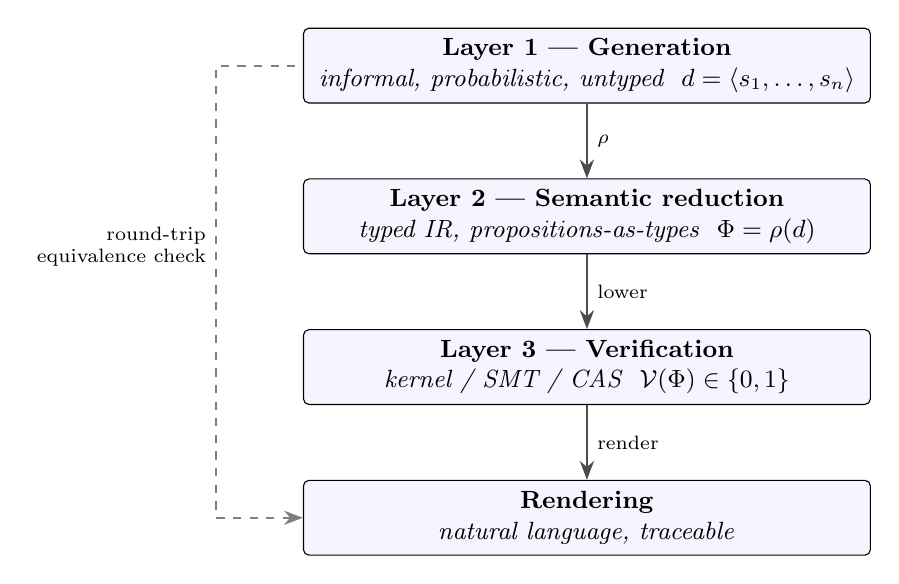
\begin{tikzpicture}[
  node distance=0.95cm,
  block/.style={rectangle, draw, rounded corners=2pt,
                minimum width=7.2cm, minimum height=0.95cm,
                align=center, font=\small, fill=blue!4},
  arrow/.style={-{Stealth[length=2.4mm]}, thick, draw=black!70},
  back/.style={{Stealth[length=2.4mm]}-, thick, dashed, draw=gray}
]
\node[block] (gen) {\textbf{Layer 1 --- Generation}\\
        \emph{informal, probabilistic, untyped}\; $d=\langle s_1,\dots,s_n\rangle$};
\node[block, below=of gen] (ir) {\textbf{Layer 2 --- Semantic reduction}\\
        \emph{typed IR, propositions-as-types}\; $\Phi=\red(d)$};
\node[block, below=of ir] (ver) {\textbf{Layer 3 --- Verification}\\
        \emph{kernel / SMT / CAS}\; $\mathcal{V}(\Phi)\in\{0,1\}$};
\node[block, below=of ver] (ren) {\textbf{Rendering}\\
        \emph{natural language, traceable}};
\draw[arrow] (gen) -- node[right, font=\scriptsize]{$\red$} (ir);
\draw[arrow] (ir)  -- node[right, font=\scriptsize]{lower} (ver);
\draw[arrow] (ver) -- node[right, font=\scriptsize]{render} (ren);
\draw[back]  (ren.west) -- ++(-1.1,0) |- (gen.west)
   node[pos=0.30, left, font=\scriptsize, align=right]
   {round-trip\\equivalence check};
\end{tikzpicture}
\caption{The three-layer architecture.  Layer~2 is the object of study in this
paper: it is the only layer whose failure is invisible to both of its
neighbours.}
\label{fig:pipeline}
\end{figure}

\subsection{Where reliability is lost}

We use two standard properties, stated so that the gap is unambiguous.

\begin{assumption}[Soundness]
$\mathcal{V}$ is \emph{sound} for $T$: $\mathcal{V}(\Phi)=1 \implies T\vdash\Phi$.
\end{assumption}

\begin{definition}[Faithful reduction]
Let $\sem{\cdot}$ denote semantic denotation.  A reduction $\red$ is
\emph{faithful} for $(c,d)$ iff $\sem{\red(d)}=\sem{c}$.  It is
\emph{sound-but-unfaithful} iff $\mathcal{V}(\red(d))=1$ but
$\sem{\red(d)}\neq\sem{c}$.
\end{definition}

\begin{proposition}[Reduction gap]
\label{prop:gap}
Suppose $\mathcal{V}$ is sound for $T$.  If $\red$ is not faithful for
$(c,d)$, then $\mathcal{V}(\red(d))=1$ does \emph{not} entail $c$ in $T$.
\end{proposition}

\begin{proof}
Soundness licenses exactly one inference: from $\mathcal{V}(\Phi)=1$ to
$T\vdash\Phi$, where $\Phi=\red(d)$.  It asserts nothing about the relation
between $\Phi$ and $c$.  By unfaithfulness, $\sem{\Phi}\neq\sem{c}$, so there
exists a structure in which $T\vdash\Phi$ holds while $c$ fails; in that
structure the pipeline outputs a certificate while the user's claim is false.
Hence no entailment from $\mathcal{V}(\Phi)=1$ to $c$ is available.
\end{proof}

Proposition~\ref{prop:gap} is almost embarrassingly simple, and that is the
point: it is the formal version of a mistake that is easy to make in practice
--- reading ``the proof checked'' as ``the claim I asked about is true''.

\begin{proposition}[Weakest-layer bound]
\label{prop:bound}
Fix a distribution of problems and a pipeline.  Let $G$, $R$ and $V$ be the
events that, on a given run, (i) the derivation $d$ is valid, (ii) the
reduction $\red(d)$ is faithful, and (iii) the verifier accepts.  Let
$\cert=G\cap R\cap V$ be the event of a genuinely certified claim, and
$p_G=\Pr(G)$, $p_R=\Pr(R)$, $p_V=\Pr(V)$.  Then
\[
  \Pr(\cert)\;\leq\;\min\{p_G,\;p_R,\;p_V\}.
\]
\end{proposition}

\begin{proof}
$\cert\subseteq G$, $\cert\subseteq R$ and $\cert\subseteq V$; apply monotonicity
of probability and take the minimum of the three bounds.
\end{proof}

\begin{remark}[Consequences]
Two practical readings follow.  First, investment in Layer~3 has \emph{zero}
effect on $\Pr(\cert)$ once $p_R$ is the binding constraint --- which is the
regime we argue the field is in.  Second, answer-level accuracy $A$ is not an
estimator of $\Pr(\cert)$: $A$ counts runs whose final answer matches a
reference, including runs with invalid reasoning.  The difference
$A-\Pr(\cert)$ is what we call the \emph{tier gap}, and it is empirically
measurable --- on GSM8K it is witnessed by the 3.4\% reasoning-error rate among
final-answer-correct solutions reported by Uesato et al.\
\cite{uesato2022process}.
\end{remark}

% =====================================================================
\section{The Semantic Reduction Bottleneck}
\label{sec:bottleneck}
% =====================================================================

\subsection{Why Layer 2}

Layer~1 fails loudly: a wrong answer is detectable by grading.  Layer~3 fails
informatively: a kernel reports the goal state, the failing tactic, the missing
hypothesis.  Layer~2 fails \emph{silently}.  Nothing in the generation layer
checks it (the prose was never checkable), and nothing in the verification
layer can see it (the kernel only ever sees $\Phi$).  Its failure modes are
therefore invisible to both neighbours and appear downstream as a puzzling
``the proof checked but the result is not what I meant''.

The literature supports placing the bottleneck here.  Autoformalisation is
treated as a research problem in its own right, with dedicated benchmarks and
baselines \cite{azerbayev2023proofnet}.  Premise selection over a library of
hundreds of thousands of declarations was identified as a key bottleneck and
addressed by retrieval \cite{yang2023leandojo}.  Large formal efforts
autoformalise tens of millions of statements to get enough training signal
\cite{hubert2025alphaproof}, and even at IMO 2024 the competition statements were
manually translated into formal language before the provers ran
\cite{hubert2025alphaproof}.  PutnamBench reports that established provers solve
only a handful of its problems \cite{tsoukalas2024putnambench} --- consistent
with a pipeline in which getting to a correct formal statement is itself a
large part of the difficulty.

\subsection{A taxonomy of reduction failures}

Table~\ref{tab:taxonomy} collects seven failure modes.  The first three were
identified in the challenge outline for this work (ambiguity, missing typing,
non-invertibility); we add four that arise from practice with real libraries.

\begin{table}[t]
\caption{A taxonomy of semantic-reduction failure modes.  ``Layer-3 signal''
  indicates whether a verifier would notice the failure on its own.}
\label{tab:taxonomy}
\centering\small
\begin{tabular}{@{}p{0.5cm}p{2.5cm}p{5.4cm}p{2.1cm}p{1.5cm}@{}}
\toprule
& \textbf{Mode} & \textbf{Description} & \textbf{Detection signal} & \textbf{Layer-3 signal}\\
\midrule
F1 & Lexical / symbolic ambiguity
  & One symbol carries two readings (e.g.\ $-$ as binary vs.\ unary; $|G|$ as order vs.\ cardinality; $\mathbb{N}$ including $0$ or not).
  & Type-checking; explicit symbol table & Yes \\
F2 & Missing typing
  & Quantified variables have no declared type or domain; implicit coercions.
  & Elaboration error & Yes \\
F3 & Non-invertibility
  & The map is many-to-one or convention-dependent; rendering back to prose is not the inverse of reduction.
  & Round-trip comparison & No \\
F4 & Premise / library mismatch
  & The invoked lemma exists but is a different result (same name, different generality) or is unavailable.
  & Premise resolution to named declarations & Partly \\
F5 & Hidden side conditions
  & Steps presuppose $x\neq 0$, convergence, compactness, non-emptiness, or a choice of branch.
  & Goal-state inspection; degenerate-case tests & Partly \\
F6 & Non-computational steps
  & Existence / choice / diagonal arguments with no computational witness.
  & Manual inspection & No \\
F7 & Round-trip drift
  & The rendered natural language no longer states $c$; readers certify the rendering, not the proof.
  & Independent equivalence judgement & No \\
\bottomrule
\end{tabular}
\end{table}

The rightmost column is the practical punchline: four of the seven modes (F3,
F6, F7, and partly F5) produce \emph{no} signal in the verification layer.  A
pipeline can therefore be perfectly sound at Layer~3 and still certify the
wrong thing.

% =====================================================================
\section{The Proposed Framework}
\label{sec:framework}
% =====================================================================

\subsection{Design of the typed IR}

We specify Layer~2 as a typed intermediate representation $\IR$ with four
components: (i) a \emph{type system} in which every quantified variable has a
declared type; (ii) an \emph{operational semantics} fixing the meaning of each
primitive, including totalised conventions (what is $x/0$? what is
$\sqrt{\cdot}$ on negatives?); (iii) a \emph{constraint system} carrying side
conditions as first-class hypotheses rather than prose; and (iv) a
\emph{compositional structure} so that partial reductions can be checked
independently.  The theoretical warrant is the propositions-as-types
correspondence \cite{wadler2015propositions}: with proofs as programs, a
reduction is a compilation step and its correctness is a typing claim, not a
matter of taste.

\subsection{Pipeline and bidirectional alignment}

The pipeline is generation $\to$ reduction $\to$ verification $\to$ rendering,
with a mandatory \emph{round-trip}: informalise $\Phi$ back to natural language
and require an independent judgement that the result is equivalent to $c$
(Figure~\ref{fig:pipeline}).  Round-tripping is not decoration --- it is the
only check that catches F3 and F7, which are otherwise undetectable.

\subsection{The Reliability Ladder}

\begin{table}[t]
\caption{The Reliability Ladder.  Tiers are ordinal: L4 subsumes L3, which
  subsumes L2, and so on.  Each tier states what a reader is entitled to
  conclude.}
\label{tab:ladder}
\centering\small
\begin{tabular}{@{}p{0.7cm}p{2.6cm}p{4.6cm}p{2.2cm}p{2.1cm}@{}}
\toprule
\textbf{Tier} & \textbf{What was done} & \textbf{What it licenses} & \textbf{Residual risk} & \textbf{Typical cost}\\
\midrule
L0 & Model produced prose & Nothing; output is a hypothesis, not a result & Unbounded & 1$\times$ \\
L1 & Self-consistency, majority voting, learned reranking \cite{cobbe2021gsm8k}
    & The output is not idiosyncratic to one sample & Correlated errors across samples & $n$$\times$ \\
L2 & External computation: calculator, CAS, numeric spot-checks \cite{schick2023toolformer,chen2022pot}
    & Numeric agreement on the tested instances & Degenerate and non-computable cases missed & 2--5$\times$ \\
L3 & Step-level process verification by a learned verifier or human step labels \cite{uesato2022process,lightman2023letsverify}
    & Each step was endorsed; errors are localised & The endorser is itself unverified & 10--100$\times$ \\
L4 & Machine-checked proof in a trusted kernel \emph{and} attested-faithful reduction \cite{moura2021lean4,hubert2025alphaproof}
    & The formal statement holds in $T$; with a faithful reduction, so does $c$ & Kernel/axiom trust; reduction faithfulness & 100--10$^4$$\times$ \\
\bottomrule
\end{tabular}
\end{table}

Table~\ref{tab:ladder} is the paper's main operational artefact.  Three
properties are worth stressing.  \emph{Monotonicity}: L4 does not replace L3,
it contains it; a serious L4 result should still report its L2 spot-checks.
\emph{Separation}: L4 is the only tier at which Prop.~\ref{prop:gap} is
defeated, because it is the only tier that explicitly attests $\sem{\red(d)}=\sem{c}$.
\emph{Cost honesty}: the rightmost column is why nobody lives at L4 by default
--- the strongest published formal results required human formalisation and, in
the IMO case, multi-day computation \cite{hubert2025alphaproof}.

\subsection{The Reduction Verification Checklist}

\begin{table}[t]
\caption{The twelve-item Reduction Verification Checklist (RVC).  Items marked
  $\ast$ are the ones we find most often skipped in practice.}
\label{tab:checklist}
\centering\small
\begin{tabular}{@{}p{0.6cm}p{7.6cm}p{3.6cm}@{}}
\toprule
& \textbf{Item} & \textbf{Failure mode caught}\\
\midrule
C1  & Every quantified variable has an explicit declared type & F2 \\
C2  & Side conditions ($x\neq 0$, convergence, compactness, non-emptiness) are explicit hypotheses & F5 \\
C3  & Every symbol has one declared meaning; overloaded notation disambiguated & F1 \\
C4  & Every invoked lemma resolves to a named declaration in the target library & F4 \\
C5$\ast$ & Library and prover versions are pinned and reported & F4 \\
C6$\ast$ & Both directions checked: formal statement $\Rightarrow$ informal claim, and conversely & F3, F7 \\
C7  & Round-trip: informalise$(\red(d))$ is judged equivalent to $c$ by an independent reader & F3, F7 \\
C8$\ast$ & Numeric spot-checks on randomly instantiated instances & F5 \\
C9  & Degenerate cases tested explicitly ($0$, $1$, $\emptyset$, boundary, $\infty$) & F5 \\
C10 & Each step is kernel-checked or explicitly flagged as assumed & F6 \\
C11$\ast$ & Provenance recorded: which parts are model-generated vs.\ human-written & F7 \\
C12$\ast$ & Acceptance rate reported over \emph{attempted} reductions, not only successful ones & all (reporting bias) \\
\bottomrule
\end{tabular}
\end{table}

Table~\ref{tab:checklist} is meant to be used as a gate: an output that fails
any of C1--C10 should not be reported above L2.

C12 deserves comment.  Reporting ``we proved 60\% of the benchmark'' is
compatible with ``we attempted 100 reductions and 40 failed silently''.  Because
Layer~2 fails silently, a denominator taken over successful reductions hides
exactly the failures this paper is about.

\subsection{A fidelity metric (proposed)}

\paragraph{Reduction Fidelity Index.}
Over $m$ checkpoints, let $r_i\in\{0,1\}$ indicate that checkpoint $i$ passed
round-trip equivalence (C7) and its spot-checks (C8--C9).  Define
\[
  \mathrm{RFI} \;=\; \frac{1}{m}\sum_{i=1}^{m} r_i .
\]
We also report, separately and never as a substitute: the reduction
\emph{acceptance rate} $a$ (fraction of attempts producing a well-typed
$\Phi$), the \emph{certified rate} $r=\Pr(\cert)$, answer-level accuracy $A$,
and the tier gap $A-r$.  RFI is a proposed metric, not a validated one; it
requires human adjudication and we do not claim it is the right weighting.

% =====================================================================
\section{Re-analysis: The Tier Gap in Published Results}
\label{sec:reanalysis}
% =====================================================================

Table~\ref{tab:reanalysis} re-reads published results through the ladder.  The
pattern is consistent: the tier that the evidence actually supports is below
the tier that the surrounding narrative invites.  We intend this as a
methodological observation, not as a criticism of the cited work, all of which
is careful about its own claims.

\begin{table}[t]
\caption{Re-analysis of published systems through the Reliability Ladder.
  ``Evidenced'' is the tier the reported artefact supports; ``Implied'' is the
  tier a reader commonly takes away.  All numbers are as reported in the cited
  source (see Appendix~\ref{app:provenance}).}
\label{tab:reanalysis}
\centering\footnotesize
\begin{tabular}{@{}p{1.9cm}p{1.9cm}p{2.5cm}p{0.9cm}p{0.9cm}p{4.4cm}@{}}
\toprule
\textbf{System} & \textbf{Artefact} & \textbf{Headline result} & \textbf{Evid.} & \textbf{Impl.} & \textbf{Why the gap}\\
\midrule
Minerva \cite{lewkowycz2022minerva}
  & MATH, STEM & SOTA without external tools & L0--L1 & L2 & Majority voting; no external check \\
Verifiers \cite{cobbe2021gsm8k}
  & GSM8K & Reranking improves accuracy & L1 & L2 & The verifier is a learned model, itself ungraded \\
Process supervision \cite{uesato2022process}
  & GSM8K & 16.8$\to$12.7\% answer error; 14.0$\to$3.4\% reasoning error & L2 & L3 & Step labels are human; no kernel \\
PRM / PRM800K \cite{lightman2023letsverify}
  & MATH subset & 78\% under best-of-$n$ & L2 & L3 & Reward model, not a proof checker \\
Toolformer, PoT \cite{schick2023toolformer,chen2022pot}
  & Arithmetic, QA & Improved zero-shot accuracy & L2 & L2 & Computation externalised; reasoning not \\
AlphaGeometry \cite{trinh2024alphageometry}
  & 30 olympiad geometry & 25 solved & L3 & L4 & Symbolic engine checks, but in a domain-specific language \\
AlphaProof \cite{hubert2025alphaproof}
  & IMO 2024 & 4/6 problems, 28/42 points & L4 & L4 & Kernel-checked, but statements formalised by humans; multi-day compute \\
Neural provers \cite{han2022minif2f,azerbayev2023proofnet,tsoukalas2024putnambench}
  & miniF2F, ProofNet, PutnamBench & Low single-digit to modest pass rates & L4 & L4 & Genuine L4 where solved; coverage is the limit \\
FunSearch \cite{romera2024funsearch}
  & Cap set, bin packing & New constructions beating known bounds & L3 & L4 & Evaluator checks programs; insight is external \\
Frontier models \cite{glazer2024frontiermath}
  & FrontierMath & Under 2\% solved & L0--L1 & L2 & Auto-verifiable answers; reasoning unexamined \\
\bottomrule
\end{tabular}
\end{table}

Two entries deserve emphasis.  \emph{AlphaProof} is the clearest L4 result in
the table, and it is precisely the case where the reduction layer was
human-staffed: the IMO statements were translated into formal language by
people before the system ran \cite{hubert2025alphaproof}.  That is not a
criticism of the system; it is a measurement of how expensive Layer~2 currently
is.  \emph{Process supervision} is the clearest measurement of the tier gap:
the 3.4\% residual reasoning error among correctly answered problems
\cite{uesato2022process} is the gap made numeric.

% =====================================================================
\section{Worked Case Study (Constructed)}
\label{sec:case}
% =====================================================================

We now exhibit the reduction gap on an elementary example.  \textbf{This
example is constructed for exposition and involves no measurement}; its
mathematics is elementary and can be checked by hand.

\paragraph{The claim.}  Consider
\[
  c:\qquad \text{``For every real number } x,\quad \frac{x^{2}-1}{x-1}=x+1.\text{''}
\]

\paragraph{A plausible generation (L0).}  A language model asked to verify $c$
typically produces something like:
\begin{quote}\small
  Factor the numerator: $x^{2}-1=(x-1)(x+1)$.  Then
  $\frac{(x-1)(x+1)}{x-1}=x+1$ after cancelling the common factor $(x-1)$.
  Hence the identity holds.
\end{quote}
The prose is fluent, the algebra is familiar, and the conclusion is
\emph{false}: at $x=1$ the left-hand side is not defined (and under the
totalised-division convention used by most proof assistants it evaluates to
$0$, while the right-hand side evaluates to $2$).  The missing step is the side
condition $x\neq 1$ --- failure mode F5.

\paragraph{Behaviour at each tier.}
\begin{itemize}[leftmargin=2.2em]
  \item \textbf{L0.}  Passes.  Nothing in the output signals a problem.
  \item \textbf{L1.}  Passes.  Independent samples produce the same
        cancellation argument, so majority voting and reranking are
        \emph{confidently} wrong: consistency is not correctness.
  \item \textbf{L2.}  Passes with high probability.  A numeric spot-check
        samples $x$ from $\mathbb{R}$; the single offending point $x=1$ has
        Lebesgue measure zero, so random testing will not find it.  This is the
        instructive part: \emph{sampling-based checking is structurally blind
        to degeneracies}, which is exactly why C9 (explicit degenerate-case
        tests) is on the checklist and not subsumed by C8.
  \item \textbf{L3.}  Flags it.  A step-level check of ``cancel $(x-1)$''
        demands the precondition $x-1\neq0$, which is absent.
  \item \textbf{L4.}  Rejects it, and in doing so reveals a second phenomenon.
\end{itemize}

\paragraph{The reduction is not unique (F3).}  Formalising $c$ requires
choosing a convention for division at zero.  In \textsf{Lean}'s field
convention division is totalised with $0^{-1}=0$, so the unconditioned
statement is simply \emph{false} and the kernel rejects it; the faithful
reduction must carry the hypothesis.  Schematically:
\begin{lstlisting}[caption={Illustrative \textsf{Lean} fragment.  Not executed
  or type-checked in this work; shown to make the side condition explicit.},
  label={lst:lean}]
-- UNFAITHFUL reduction: no side condition. This statement is FALSE at x = 1.
theorem bad (x : R) : (x^2 - 1) / (x - 1) = x + 1 := by
  ring_nf          -- fails: the goal is false at x = 1

-- FAITHFUL reduction: the hidden side condition is now a hypothesis.
theorem good (x : R) (hx : x <> 1) : (x^2 - 1) / (x - 1) = x + 1 := by
  have h : x - 1 <> 0 := sub_ne_zero.mpr hx
  field_simp [h]
  ring
\end{lstlisting}
The same English sentence therefore reduces to two formal statements with
\emph{different truth values}, depending on a convention the prose never
mentions.  That is non-invertibility in the sense of F3, and it is invisible to
Layer~3: the kernel is impeccably correct in both cases.  It is only visible if
someone performs C6 (check both directions) and C7 (round-trip).

\paragraph{What the case study shows.}  Three things, in order of importance:
(1) tiers L0--L2 can all pass on a false claim, and L1 can pass
\emph{confidently}; (2) the failure is undetectable by random numeric testing
because the failure set has measure zero; and (3) the reduction step is
convention-dependent, so ``the formal statement'' is not uniquely determined by
the English --- which is precisely the situation Proposition~\ref{prop:gap}
describes.

% =====================================================================
\section{A Pre-specified Protocol for Measuring Reduction Fidelity}
\label{sec:protocol}
% =====================================================================

We close the methodological loop by pre-specifying how the framework would be
tested.  \textbf{This protocol is not executed in this paper}; we give it so
that the framework is falsifiable and so that the required sample size is
visible in advance.

\paragraph{Corpus.}  Use ProofNet \cite{azerbayev2023proofnet} as the primary
instrument: its 371 items each pair a natural-language statement, a natural-language
proof, and a reference formal statement, which supplies a \emph{gold} target
against which reduction fidelity can be scored rather than merely asserted.
miniF2F \cite{han2022minif2f} (488 statements) and PutnamBench
\cite{tsoukalas2024putnambench} provide harder and broader secondary corpora.

\paragraph{Procedure.}  For each item $i$: (1) a generator produces an informal
derivation $d_i$; (2) a reduction module (model plus deterministic compiler)
produces $\Phi_i$; (3) fidelity is adjudicated by comparing $\Phi_i$ to the gold
formal statement, using definitional equality where available and two
independent human adjudicators otherwise; (4) a kernel check is attempted and
the goal state recorded; (5) checklist C8--C9 spot-checks are run.

\paragraph{Reported quantities.}  Reduction acceptance rate $a$; RFI;
answer-level accuracy $A$; certified rate $r$; tier gap $A-r$; and the
conditional gap given document-style fluency, $A-r$ restricted to outputs an
expert rates as plausible.  The last quantity is the one that matters most for
users: it is the probability that a plausible-looking answer is wrong.

\paragraph{Sample size.}  For a two-proportion comparison at $\alpha=0.05$,
power $0.80$, with $p_1=0.5$, $p_2=0.4$ and $\delta=0.10$,
\[
  n \;\approx\; \frac{(z_{0.975}+z_{0.80})^{2}\,\bigl(p_1(1-p_1)+p_2(1-p_2)\bigr)}{\delta^{2}}
  \;\approx\; 385 \;\text{items}.
\]
ProofNet's 371 items are therefore adequate for detecting a ten-point gap and
\emph{under-powered} for smaller ones --- which is worth stating in advance,
because a null result on 371 items would not license the conclusion that
reduction is faithful.

\paragraph{Falsification.}  The framework's central empirical claim is that
$p_R$ is the binding constraint in Proposition~\ref{prop:bound}.  It would be
refuted by a study in which, on a non-trivial corpus, reduction acceptance $a$
and fidelity are both high while certified rate $r$ remains low --- i.e.\ the
binding constraint sits at Layer~1 or Layer~3 after all.

% =====================================================================
\section{Threats to Validity and Limitations}
\label{sec:limits}
% =====================================================================

\begin{itemize}[leftmargin=2.2em]
  \item \textbf{No new empirical results.}  Section~\ref{sec:case} is
        constructed; Section~\ref{sec:protocol} is unexecuted.  The framework's
        empirical claim is stated as a hypothesis with a falsification
        condition, not as a finding.
  \item \textbf{Faithfulness has no formal ground in general.}  $\sem{c}$
        presupposes a semantics for informal mathematical language, which does
        not exist in general.  We operationalise faithfulness against gold
        formalisations and human adjudication
        (Section~\ref{sec:protocol}); this makes the notion usable but leaves it
        partly judgement-dependent.
  \item \textbf{The ladder is ordinal.}  L4 is not ``four times L1''.  Tier
        assignments in Table~\ref{tab:reanalysis} involve interpretation, and
        reasonable readers may disagree at the margin; we have tried to state
        the basis for each assignment in the final column.
  \item \textbf{Kernel and library trust.}  L4 assumes the proof checker, its
        axiomatisation, and the library are correct.  A large trusted base
        \cite{mathlib2020} is a real assumption, not a formality.
  \item \textbf{Cost.}  L4 is expensive in human effort and compute
        \cite{hubert2025alphaproof}.  Our argument is that the ladder should be
        reported honestly, not that everyone should live at L4.
  \item \textbf{A moving field.}  All reported numbers are as of the cited
        publications and were re-checked on 2026-09-25; several benchmarks are
        actively being saturated.
\end{itemize}

% =====================================================================
\section{Conclusion}
\label{sec:conclusion}
% =====================================================================

Reliability in AI mathematics is not a property of a model; it is a property of
a pipeline, and pipelines have three layers.  We argued that the middle one ---
semantic reduction, the map from informal argument to checkable object --- is
where reliability is most often lost, because it is the only layer whose
failures are invisible to both of its neighbours.  Proposition~\ref{prop:gap}
shows that a sound verifier certifies the reduced object and not the user's
claim; Proposition~\ref{prop:bound} shows that effort spent on generation or
verification is wasted while reduction is the binding constraint.  We
contributed a Reliability Ladder and a Reduction Verification Checklist so that
this can be audited rather than asserted, re-read the recent literature through
them to expose a systematic tier gap, and pre-specified a protocol for
measuring reduction fidelity.

The practical recommendation is modest and cheap: \emph{publish the tier}.  A
result reported as ``78\% on a MATH subset'' and the same result reported as
``78\% at L2, with no kernel-checked proof and no round-trip verification''
are different scientific objects.  Making the tier explicit costs a sentence
and removes most of the ambiguity that this paper has tried to describe.

% =====================================================================
\appendix
\section{Provenance and Verification Record}
\label{app:provenance}
% =====================================================================

Every external quantitative claim in this paper was checked against its source
on 2026-09-25.  This appendix records the check so that the claims can be
audited independently.  \emph{Verification method} describes how the claim was
confirmed: \textbf{P} = publisher/primary page, \textbf{A} = arXiv abstract
page, \textbf{S} = authoritative secondary index (ADS, PubMed, DBLP, or a
publisher-hosted citation record).

\begin{table}[htbp]
\centering\footnotesize
\begin{tabular}{@{}p{5.2cm}p{1.6cm}p{1.7cm}p{2.4cm}p{1.6cm}@{}}
\toprule
\textbf{Claim as used in this paper} & \textbf{Source} & \textbf{Method} & \textbf{Outcome} & \textbf{Status}\\
\midrule
AlphaProof: 4/6 IMO 2024 problems, 28/42 points, silver-medal equivalent & \cite{hubert2025alphaproof} & P + A (PMC full text) & Confirmed & OK \\
IMO 2024 statements were manually translated into formal language for the system & \cite{hubert2025alphaproof} & P (press release, PMC) & Confirmed & OK \\
AlphaProof trained on $\sim$80M autoformalised problems & \cite{hubert2025alphaproof} & P (press release) & Confirmed & OK \\
AlphaGeometry solves 25 of 30 olympiad geometry problems & \cite{trinh2024alphageometry} & P & Confirmed & OK \\
miniF2F: 488 problem statements & \cite{han2022minif2f} & A + P (ICLR) & Confirmed & OK \\
ProofNet: 371 examples & \cite{azerbayev2023proofnet} & A + P (repo) & Confirmed; journal version \emph{not} confirmed & Cited as preprint \\
PutnamBench: 1692 formalisations, 640 theorems; provers solve a handful & \cite{tsoukalas2024putnambench} & A & Confirmed & OK \\
LeanDojo: 98,734 theorems; premise retrieval & \cite{yang2023leandojo} & A + P (NeurIPS) & Confirmed & OK \\
MATH: 12,500 problems & \cite{hendrycks2021math} & A + P & Confirmed & OK \\
GSM8K: 8.5K problems & \cite{cobbe2021gsm8k} & A (ADS) & Confirmed & OK \\
16.8$\to$12.7\% answer error; 14.0$\to$3.4\% reasoning error & \cite{uesato2022process} & A (arXiv PDF) & Confirmed verbatim & OK \\
PRM: 78\% of a MATH subset; PRM800K labels & \cite{lightman2023letsverify} & A (ADS + arXiv) & Confirmed & OK \\
FrontierMath: models solve under 2\% & \cite{glazer2024frontiermath} & A & Confirmed & OK \\
FunSearch: new cap-set constructions; Nature 625:468--475 & \cite{romera2024funsearch} & P & Confirmed & OK \\
Lean 4: CADE 28, LNCS 12699, pp.\ 625--635 & \cite{moura2021lean4} & P (Springer/KIT) & Confirmed & OK \\
mathlib: CPP 2020, pp.\ 367--381 & \cite{mathlib2020} & S (cited record in \cite{moura2021lean4}) & Confirmed & OK \\
Toolformer: NeurIPS 36, pp.\ 68539--68551 & \cite{schick2023toolformer} & S (Scholar/NeurIPS) & Confirmed & OK \\
Lean's totalised division ($0^{-1}=0$) makes the unconditioned identity false at $x=1$
  & \cite{moura2021lean4,mathlib2020} & Derived by hand & Convention-dependent; stated as such in \S\ref{sec:case} & Qualified \\
\bottomrule
\end{tabular}
\end{table}

\paragraph{Declared corrections.}  Two items were adjusted during verification
and are recorded here rather than silently fixed:
\begin{enumerate}[label=(\arabic*),leftmargin=2.2em]
  \item ProofNet is cited as an arXiv preprint.  A journal version (TMLR) was
        suggested during drafting but could not be confirmed, so no journal
        venue is claimed.
  \item The AlphaProof Nature paper is cited by DOI only.  Volume and page
        numbers were not confirmed at the time of writing and have not been
        invented.
\end{enumerate}

\paragraph{AI-assisted provenance.}  Parts of this manuscript were drafted with
the assistance of a language model.  All literature claims were subsequently
verified against sources by the author; the per-claim record is the table
above, and the day-by-day collaboration record --- including cases where the
model produced an incorrect claim that was caught in verification --- is shipped
with this manuscript as the accompanying AI collaboration log and after-action
review.

% =====================================================================
\bibliographystyle{plain}
\bibliography{references}
% =====================================================================

\end{document}
